\section{Instrukcja obsługi programu}

\subsection{Uruchomienie}

Program jest jednym plikiem wykonywalnym \code{empirical-reliability.exe} (Windows 10/11,
64 bity). Nie wymaga instalacji ani dodatkowych plików -- wystarczy go uruchomić.
Do działania potrzebny jest sterownik karty graficznej z~obsługą OpenGL, dostępny
standardowo w~systemie. Wersję dla systemu Linux lub macOS buduje się z~kodu
źródłowego (p.~\ref{sec:build}).

\subsection{Okno programu}

Okno jest podzielone na dwie części (rys.~\ref{fig:start}). Po lewej stronie
wprowadza się dane w~jednej z~trzech zakładek: ,,Próba losowa'', ,,Tabela uszkodzeń''
albo ,,Lista czasów''. Po prawej stronie znajdują się wyniki w~zakładkach ,,Wyniki'',
,,Wykresy'' i~,,Próba''. Granicę między częściami można przesuwać myszą.

Liczby można wpisywać z~przecinkiem albo z~kropką dziesiętną (np. \code{0,01} lub
\code{0.01}). Każde obliczenie zastępuje poprzednie wyniki.

\begin{figure}[H]
  \centering
  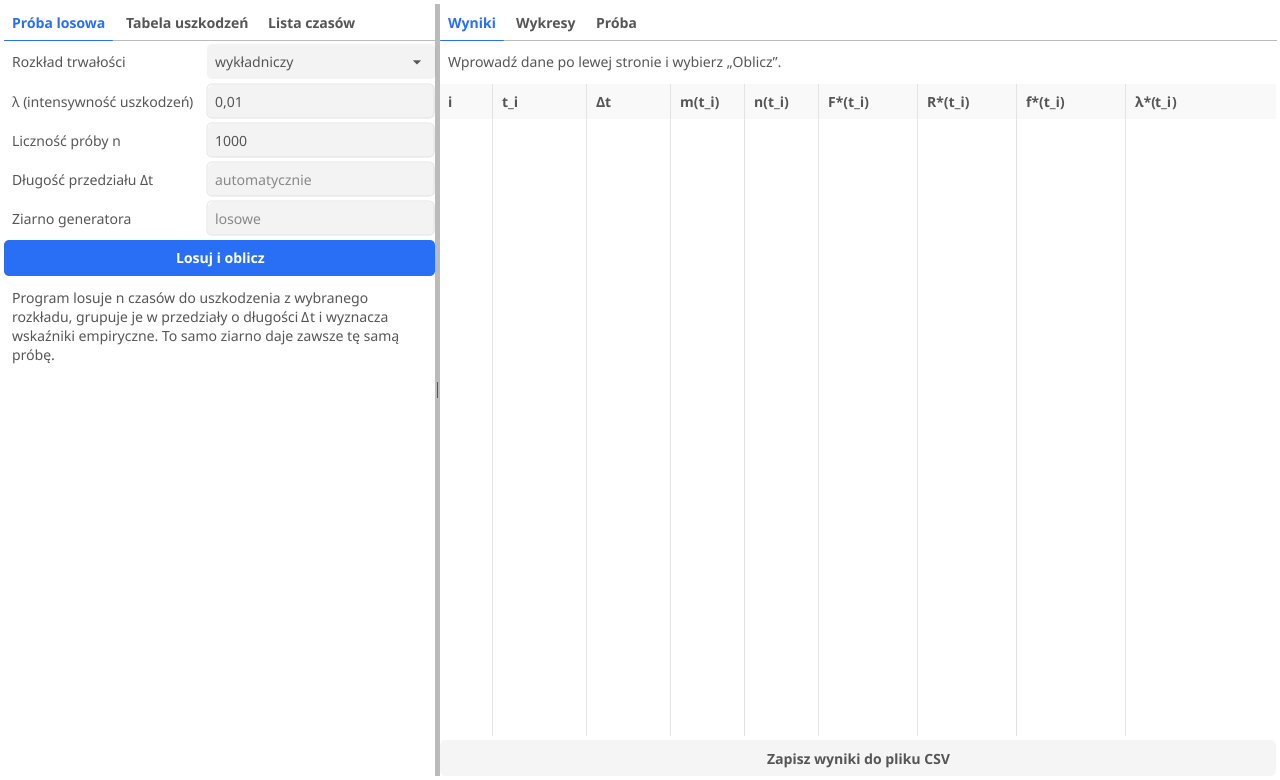
\includegraphics[width=\textwidth]{01_start}
  \caption{Okno programu po uruchomieniu}
  \label{fig:start}
\end{figure}

\subsection{Próba losowa}

Zakładka służy do wylosowania czasów do uszkodzenia z~rozkładu teoretycznego.
\begin{enumerate}
  \item Wybrać \textbf{rozkład trwałości}: wykładniczy, Weibulla albo normalny.
  \item Podać \textbf{parametry rozkładu} -- pola zmieniają się zależnie od rozkładu
    i~są wypełnione wartościami domyślnymi: $\lambda$ dla wykładniczego; $\beta$
    (kształt) i~$\eta$ (skala) dla Weibulla; $\mu$ i~$\sigma$ dla normalnego.
    Wszystkie parametry muszą być dodatnie.
  \item Podać \textbf{liczność próby $n$} (od 1 do 1\,000\,000).
  \item Opcjonalnie podać \textbf{długość przedziału $\Delta t$}. Puste pole oznacza
    dobór automatyczny.
  \item Opcjonalnie podać \textbf{ziarno generatora} (nieujemna liczba całkowita).
    To samo ziarno daje zawsze tę samą próbę; przy pustym polu każde losowanie jest
    inne, a~użyte ziarno jest pokazywane w~podsumowaniu wyników.
  \item Nacisnąć \textbf{,,Losuj i~oblicz''}.
\end{enumerate}

\subsection{Tabela uszkodzeń}

Zakładka służy do wprowadzenia danych pogrupowanych, takich jak w~przykładach
z~książki.
\begin{enumerate}
  \item Podać \textbf{liczność próby $n(0)$}.
  \item W~polu tekstowym wpisać tabelę: w~każdym wierszu chwilę $t$ oraz liczbę
    elementów uszkodzonych $m(t)$ zarejestrowaną w~tej chwili, rozdzielone spacją,
    tabulatorem lub średnikiem, np. \code{2 3}. Chwile muszą być dodatnie i~rosnące,
    ale odstępy między nimi nie muszą być równe. Puste wiersze są pomijane.
  \item Nacisnąć \textbf{,,Oblicz''}.
\end{enumerate}
Suma uszkodzeń może być mniejsza od $n(0)$ -- pozostałe elementy są wtedy traktowane
jako zdatne po zakończeniu obserwacji. Przycisk ,,Przykład z~książki'' wczytuje dane
z~przykładu 5.1, a~,,Wyczyść'' usuwa zawartość formularza.

\subsection{Lista czasów}

Zakładka służy do wprowadzenia pojedynczych czasów uszkodzeń.
\begin{enumerate}
  \item W~polu tekstowym wpisać czasy do uszkodzenia kolejnych elementów, rozdzielone
    spacjami, średnikami lub znakami nowej linii, w~dowolnej kolejności.
  \item Opcjonalnie podać \textbf{liczność próby $n(0)$}. Puste pole oznacza, że
    liczność jest równa liczbie podanych czasów. Jeżeli $n(0)$ jest większe, pozostałe
    elementy są traktowane jako zdatne do końca obserwacji.
  \item Opcjonalnie podać \textbf{długość przedziału $\Delta t$}.
  \item Nacisnąć \textbf{,,Oblicz''}.
\end{enumerate}

\subsection{Wyniki}

Zakładka ,,Wyniki'' (rys.~\ref{fig:random-results}) zawiera podsumowanie i~tabelę.
W~podsumowaniu podane są: liczność próby, liczba przedziałów i~czas obserwacji,
liczba elementów uszkodzonych i~zdatnych, $E^*T$ ze wzoru (5-15) oraz $E^*T$
z~funkcji $R^*(t)$, a~dla próby losowej także rozkład, jego parametry, użyte ziarno
i~teoretyczna wartość oczekiwana $ET$. Kolumny tabeli opisano w~tab.~\ref{tab:columns}.

\begin{table}[H]
  \centering
  \caption{Kolumny tabeli wyników}
  \label{tab:columns}
  \small
  \begin{tabular}{@{}ll@{}}
    \toprule
    Kolumna & Znaczenie \\
    \midrule
    $i$ & numer przedziału \\
    $t_i$ & koniec przedziału (chwila rejestracji) \\
    $\Delta t$ & długość przedziału \\
    $m(t_i)$ & liczba elementów uszkodzonych w~przedziale \\
    $n(t_i)$ & liczba elementów zdatnych w~chwili $t_i$ \\
    $F^*(t_i)$ & dystrybuanta empiryczna \\
    $R^*(t_i)$ & empiryczna funkcja niezawodności \\
    $f^*(t_i)$ & empiryczna gęstość prawdopodobieństwa \\
    $\lambda^*(t_i)$ & empiryczna intensywność uszkodzeń \\
    \bottomrule
  \end{tabular}
\end{table}

Znak ,,---'' w~kolumnie $\lambda^*(t_i)$ oznacza wartość nieokreśloną: na początku
przedziału nie było już elementów zdatnych. Jeżeli nie wszystkie elementy uległy
uszkodzeniu, $E^*T$ ze wzoru (5-15) nie jest wyznaczana, a~wartość z~funkcji $R^*(t)$
jest oszacowaniem od dołu.

\begin{figure}[H]
  \centering
  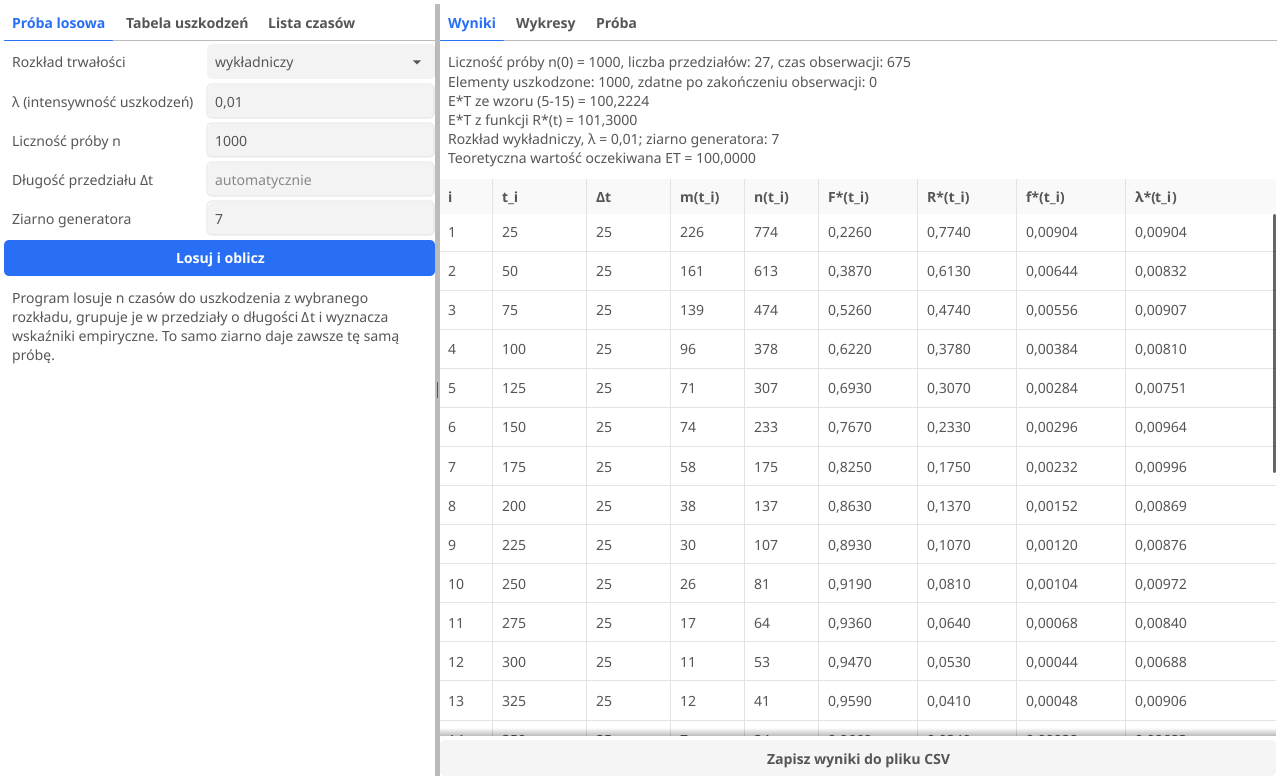
\includegraphics[width=\textwidth]{04_random_results}
  \caption{Zakładka ,,Wyniki'' dla próby losowej}
  \label{fig:random-results}
\end{figure}

\subsection{Wykresy}

Zakładka ,,Wykresy'' (rys.~\ref{fig:random-charts}) pokazuje przebiegi $F^*(t)$,
$R^*(t)$, $f^*(t)$ i~$\lambda^*(t)$. Dystrybuanta i~funkcja niezawodności są
narysowane jako punkty w~chwilach $t_i$ połączone odcinkami. Gęstość i~intensywność
uszkodzeń dotyczą całych przedziałów, dlatego są narysowane jako wykresy schodkowe.
Dla próby losowej czerwona linia przerywana pokazuje przebieg teoretyczny rozkładu,
z~którego losowano.

\begin{figure}[H]
  \centering
  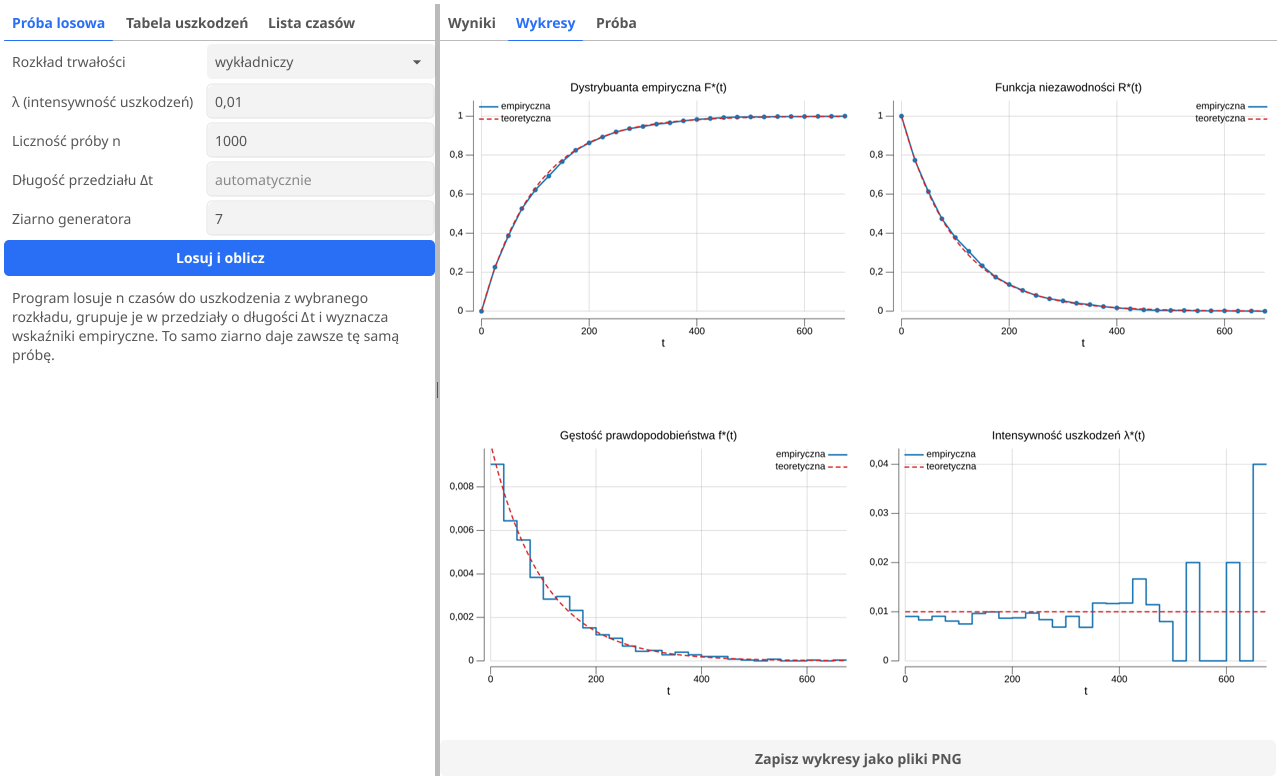
\includegraphics[width=\textwidth]{05_random_charts}
  \caption{Zakładka ,,Wykresy'' dla próby losowej}
  \label{fig:random-charts}
\end{figure}

\subsection{Próba}

Zakładka ,,Próba'' (rys.~\ref{fig:random-sample}) zawiera pojedyncze czasy uszkodzeń
posortowane rosnąco -- wylosowane albo wpisane w~zakładce ,,Lista czasów''. Można je
zaznaczyć i~skopiować, na przykład po to, by wkleić je do zakładki ,,Lista czasów''
i~przeliczyć z~inną długością przedziału. Dla danych z~tabeli uszkodzeń zakładka jest
pusta, ponieważ pojedyncze czasy nie są wtedy znane.

\begin{figure}[H]
  \centering
  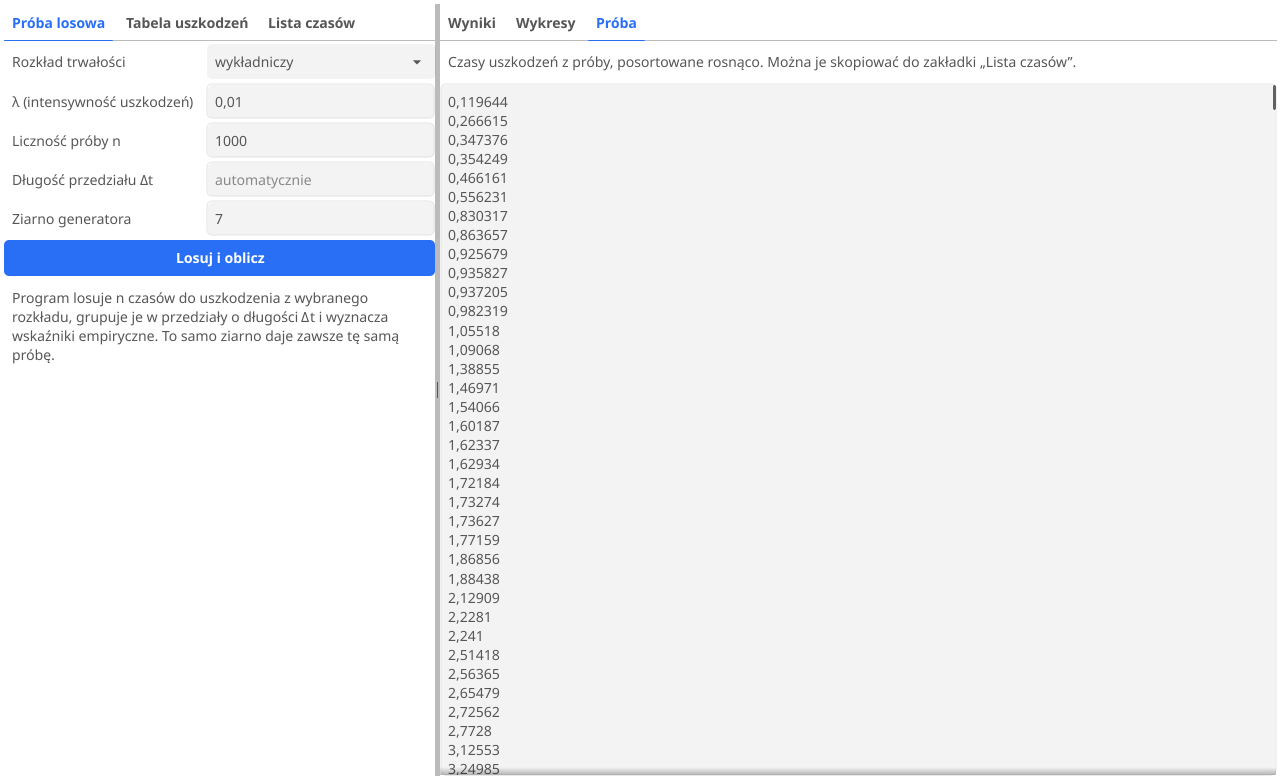
\includegraphics[width=\textwidth]{06_random_sample}
  \caption{Zakładka ,,Próba'' z~wylosowanymi czasami}
  \label{fig:random-sample}
\end{figure}

\subsection{Zapis wyników}

\begin{itemize}
  \item \textbf{,,Zapisz wyniki do pliku CSV''} (zakładka ,,Wyniki'') zapisuje tabelę
    wyników oraz wartości $n(0)$ i~$E^*T$. Plik ma domyślną nazwę \code{results.csv},
    średnik jako separator kolumn i~przecinek dziesiętny, więc otwiera się
    bezpośrednio w~polskiej wersji programu Excel.
  \item \textbf{,,Zapisz wykresy jako pliki PNG''} (zakładka ,,Wykresy'') zapisuje
    cztery wykresy do wskazanego folderu jako \code{cdf.png} (dystrybuanta),
    \code{reliability.png} (funkcja niezawodności), \code{density.png} (gęstość)
    i~\code{hazard.png} (intensywność uszkodzeń).
\end{itemize}
Oba przyciski działają dopiero po wykonaniu obliczeń.

\subsection{Komunikaty o~błędach}

Jeżeli dane są niepoprawne, program wyświetla okno z~opisem błędu (rys.~\ref{fig:error})
i~nie zmienia wyników. Komunikat wskazuje pole formularza, numer wiersza tabeli albo
pozycję na liście czasów, w~której wykryto błąd. Po zamknięciu okna przyciskiem
,,OK'' należy poprawić dane i~ponowić obliczenia. Przykłady komunikatów zawiera
tab.~\ref{tab:errors}.

\subsection{Budowanie programu z~kodu źródłowego}
\label{sec:build}

Do zbudowania programu potrzebne są: Go w~wersji 1.26 lub nowszej oraz kompilator
języka C, którego wymaga biblioteka Fyne. Plik wykonywalny buduje się na tym
systemie, na którym ma działać, poleceniem wydanym w~katalogu głównym programu
(tab.~\ref{tab:build}). Wynikiem jest zawsze jeden plik wykonywalny.

\begin{table}[H]
  \centering
  \caption{Budowanie programu w~poszczególnych systemach}
  \label{tab:build}
  \small
  \begin{tabular}{@{}l>{\raggedright\arraybackslash}p{0.3\textwidth}>{\raggedright\arraybackslash}p{0.48\textwidth}@{}}
    \toprule
    System & Dodatkowe wymagania & Polecenie \\
    \midrule
    Windows & gcc (MinGW-w64) &
      \code{go build -ldflags "-H=windowsgui -s -w" -o empirical-reliability.exe .} \\
    Linux & pakiety \code{gcc}, \code{libgl1-mesa-dev}, \code{xorg-dev}, \code{libxkbcommon-dev}, \code{libwayland-dev} &
      \code{go build -ldflags "-s -w" -o empirical-reliability .} \\
    macOS & narzędzia wiersza poleceń Xcode &
      \code{go build -ldflags "-s -w" -o empirical-reliability .} \\
    \bottomrule
  \end{tabular}
\end{table}
